\documentclass[12pt]{extarticle}
\usepackage{geometry}
\geometry{
a4paper,
total={170mm,257mm},
left=20mm,
top=20mm,
headheight=12pt
}

\usepackage[parfill]{parskip} % Activate to begin paragraphs with an empty line rather than an indent
\usepackage{graphicx} % Use pdf, png, jpg, or eps§ with pdflatex; use eps in DVI mode
% TeX will automatically convert eps --> pdf in pdflatex
\graphicspath{ {./Figures/} }
\usepackage{subcaption}
\usepackage{float}

\usepackage{amssymb,amsmath,amsthm}
\usepackage{commath}
\usepackage[hyphens]{url}
\usepackage[dvipsnames]{xcolor}
\usepackage[unicode=true,colorlinks=true,urlcolor=CadetBlue,citecolor=black,linkcolor=black]{hyperref}
\PassOptionsToPackage{hyphens}{url} % url is loaded by hyperref
\usepackage{authblk}
\usepackage{longtable}
\usepackage{multirow}
\usepackage{booktabs}
\usepackage{lipsum}  
\usepackage[title,page]{appendix}
\usepackage{chngcntr}
      
%SetFonts
% newtxtext+newtxmath
\usepackage{newtxtext} %loads helv for ss, txtt for tt
\usepackage{amsmath}
\usepackage[bigdelims]{newtxmath}
\usepackage[T1]{fontenc}
\usepackage{textcomp}
%SetFonts

% less space before sections 
% \@startsection {NAME}{LEVEL}{INDENT}{BEFORESKIP}{AFTERSKIP}{STYLE} 
%            optional * [ALTHEADING]{HEADING} 
\makeatletter
 \renewcommand\section{\@startsection {section}{1}{\z@}%
     {-2.5ex \@plus -1ex \@minus -.2ex}%
     {1.3ex \@plus.2ex}%
    {\Large\bfseries}}
    
% Species names
%% Meta-Command for defining new species macros
\usepackage{xspace}

\newcommand{\species}[3]{%
  \newcommand{#1}{\gdef#1{\textit{#3}\xspace}\textit{#2}\xspace}}
  
\species{\yeast}{Saccharomyces cerevisiae}{S.~cerevisiae}
\species{\calbicans}{Candida albicans}{C.~albicans}
\species{\cneoformans}{Cryptococcus neoformans}{C.~neoformans}

% line numbers
 \usepackage[displaymath, mathlines]{lineno}
 \renewcommand\linenumberfont{\normalfont\small\sffamily}
\linenumbers
\modulolinenumbers[2]

% Yoav & Lee commands
\newcommand*{\tr}{^\intercal}
\let\vec\mathbf
\newcommand{\matrx}[1]{{\left[ \stackrel{}{#1}\right]}}
\newcommand{\diag}[1]{\mbox{diag}\matrx{#1}}
\newcommand{\goesto}{\rightarrow}
\newcommand{\dspfrac}[2]{\frac{\displaystyle #1}{\displaystyle #2} }
\newtheorem{theorem}{Theorem}
\newtheorem{corollary}{Corollary}
\newtheorem{lemma}{Lemma}
\newtheorem{remark}{Remark}
\newtheorem{result}{Result}
\renewcommand\qedsymbol{} % no square at end of proof
\newcommand{\cl}{\mathbf{L}}
\newcommand{\cj}{\mathbf{J}}
\newcommand{\ci}{I}

% Supplementary
% https://support.authorea.com/en-us/article/how-to-create-an-appendix-section-or-supplementary-information-1g25i5a/
\newcommand{\beginsupplement}{%
      	\setcounter{table}{0}
        \renewcommand{\thetable}{S\arabic{table}}%
        \setcounter{figure}{0}
        \renewcommand{\thefigure}{S\arabic{figure}}%
		\setcounter{equation}{0}
        \renewcommand{\theequation}{A\arabic{equation}}%
}

% NatBib
\usepackage[round,colon]{natbib}

% Title page
\title{Cultural Transmission Can Explain the Evolution of Cooperation}

% Authors
\renewcommand\Affilfont{\small}

\author[1]{Dor Cohen}
\author[2]{Ohad Lewin-Epstein}
\author[3]{Marcus W. Feldman}
\author[a,*]{Yoav Ram}

\affil[1]{School of Computer Science, Interdisciplinary Center Herzliya, Herzliya, Israel}
\affil[2]{School of Plant Sciences and Food Security, Tel Aviv University, Tel Aviv, Israel}
\affil[3]{Department of Biology, Stanford University, Stanford, CA}
\affil[*]{Corresponding author: yoav@yoavram.com}

\date{\today}

\begin{document}
\maketitle

% Abstract
%\begin{abstract}
%\end{abstract}

\pagebreak


%%%%%%%%%%%%%%%%%%%%%%%%%%%
%%% Introduction
\section*{Introduction}
Cooperative behavior can reduce an individual's fitness and increase the fitness of its conspecifics or competitors~\citep{axelrod1981evolution}.
Nevertheless, cooperative behavior appears to occur in many non-human animals~\citep{dugatkin1997cooperation}, including primates~\citep{jaeggi2013natural},  rats~\citep{rice1962altruism}, birds~\citep{stacey1990cooperative,krams2008experimental}, and lizards~\citep{sinervo2006self}.
Evolution of cooperative behavior remains an important conundrum in evolutionary biology. Since the work of  \citet{hamilton1964genetical} and \citet{axelrod1981evolution}, theories for the evolution of cooperative and altruistic behaviors have been intertwined often under the rubric of kin selection.

\emph{Kin selection} theory posits that natural selection is more likely to favor cooperation between more closely related individuals. The importance of relatedness to the evolution of cooperation and altruism was shown by~\citet{hamilton1964genetical}, who showed that an allele that determines cooperative behavior will increase in frequency if the reproductive cost to the actor that cooperates, $c$, is less than the benefit to the recipient, $b$, times the relatedness, $r$, between the recipient and the actor. This relatedness coefficient $r$ measures a probability that an allele sampled from the cooperator is identical by descent to one at the same locus in the recipient.
This condition is  known as ``Hamilton's rule'':
\begin{equation} \label{eq:hamilton_rule}
c < b \cdot r.
\end{equation}

\citet{Eshel1982}  studied a related model for the evolution of cooperative behavior under vertical transmission. Their model included \emph{assortative meeting}, or non-random encounters, where a fraction $m$ of individuals in the population each interact with an individual of the same phenotype, and a fraction $1-m$ interacts  with a randomly chosen individual.  
Such assortative meeting may be due, for example, to population structure or active partner choice.
In their model, cooperative behavior can evolve if\footnote{In an extended model, which allows an individual to encounter $N$ individuals before choosing a partner, the righthand side is multiplied by $E[N]$, the expected number of encounters \citep[eq.~4.6]{Eshel1982}.
} 
\citep[eq.~3.2]{Eshel1982}
\begin{equation} \label{eq:assortative_meeting}
c < b \cdot m\,,
\end{equation}
where $b$ and $c$ are the benefit and cost of cooperation. 
Here $m$ in (\ref{eq:assortative_meeting}) takes the role of the relatedness $r$  in (\ref{eq:hamilton_rule}).


%These theories assume that cooperation is genetically determined, which raises the question: \emph{Is it possible that cooperation is determined by non-genetic factors?}
%Culture has significant impact on the behavior of humans~\citep{ihara2004cultural,jeong2018bronze} as well as non-human animals~\citep{bonner2018evolution}.

Here we study the evolution of a cooperative behavior that is subject to \emph{cultural transmission},
 which allows an individual to acquire attitudes or behavioral traits from other individuals in its social group through imitation, learning, or other modes of communication \citep{cavalli1981cultural,richerson2008not}.
\citet{feldman1985gene} introduced the first model for the evolution of altruism by cultural transmission and
showed that under vertical (parent-to-offspring) cultural transmission, the conditions for the initial increase of altruism entails a modification of Hamilton's rule in the cases  of parent-to-offspring or sib-to-sib altruism.

\emph{Non-vertical cultural transmission} may be either viewed as horizontal or oblique: horizontal transmission occurs between individuals from the same generation, while oblique transmission occurs  to  offspring from the generation to which their parents belong. 
Evolution under either of these transmission models  can be be more rapid than under pure vertical transmission~\citep{cavalli1981cultural,lycett2008questions,ram2018evolution}.
\citet{lewin2017microbes} have demonstrated that non-vertical transmission, mediated by microbes that manipulate their host's behavior, can help to explain the evolution of cooperative behavior. Some of their analysis can be applied to cultural transmission, because models of cultural transmission are mathematically similar to those for transmission of infectious diseases~\citep{cavalli1981cultural}.

We hypothesize that non-vertical cultural transmission can enhance the evolution of cooperation, and 
to test this hypothesis we suggest a model in which behavioral changes are mediated by cultural transmission that can occur during social interactions. For example, if an individual interacts with a cooperative individual, it might learn that cooperation is an advantageous behavior and will be cooperative in the future. 
Our cultural evolution models  include both vertical and non-vertical transmission of cooperation, and we investigate these models using mathematical analysis and simulations.  
Our results demonstrate that cultural transmission can facilitate the evolution of cooperation even when genetic transmission can not, and that treatment of cooperation as a cultural, rather than a genetic, trait can lead to a better understanding of its evolutionary dynamics.


%%%%%%%%%%%%%%%%%%%%%%%%%%%
% Models
\section*{Models}

Consider a very large population whose members are characterized by their phenotype $\phi$, which can be of two types, $\phi=A$ for cooperators or $\phi=B$ for defectors.
An offspring inherits its phenotype from its parent via vertical transmission with probability $v$ or from a random individual in the parental population via oblique transmission with probability $(1-v)$. 
Following~\citet{ram2018evolution}, given that the parent phenotype is $\phi$ and assuming uni-parental inheritance, % yr: cite Zefferman Behav Ecol 2016
the conditional probability that the phenotype $\phi'$ of the offspring is $A$ is 

\begin{equation} \label{eq:vertical_oblique_transmission}
P(\phi'=A \mid \phi) = \begin{cases}
v + (1-v)p, & \text{if } \phi=A \\
(1-v)p, & \text{if } \phi=B
\end{cases},
\end{equation}
where $p=P(\phi=A)$ is the frequency of $A$ among all adults in the parental generation.  

Not all adults become parents due to natural selection, and we denote the frequency of phenotype $A$ among parents by $\tilde{p}$.
Therefore, the frequency $\hat{p}$ of  phenotype $A$ among juveniles (after selection and vertical and oblique transmission) is

\begin{equation}\label{eq:horizontal}
\begin{aligned}
\hat{p}
& = \tilde{p} [v + (1-v)p] + (1-\tilde{p}) [(1-v)p] \\
& = v \tilde{p} + (1-v) p.
\end{aligned}
\end{equation}

Individuals are assumed to interact according to a \emph{prisoner's dilemma}.
Specifically, individuals interact in pairs; a cooperator suffers a fitness cost $0<c<1$, and its partner gains a fitness benefit $b$, where we assume $c<b$. \textbf{\autoref{table:prisoner_payoff}} shows the payoff matrix, i.e. the fitness of an individual with phenotype $\phi_1$ when interacting with a partner of phenotype $\phi_2$.

\bigskip
\begin{center}[TABLE 1 HERE]\end{center}
%%% Table: payoff matrix


\bigskip
Social interactions occur randomly:
two individuals with phenotype $A$ interact with probability $\hat{p}^2$, two individuals with phenotype $B$ interact with probability $(1-\hat{p})^2$, and two individuals with different phenotypes interact with probability $2\hat{p}(1-\hat{p})$. 

Horizontal cultural transmission occurs between pairs of individuals from the same generation. 
It occurs between social partners with probability $\alpha$, or between a random pair with probability $1-\alpha$ (see~\textbf{\autoref{fig:horizontal}}).
The assortment parameter $\alpha$ is therefore the fraction of population that receives (horizontal transmission) from the social interaction partner, and $1-\alpha$ receives randomly.
Horizontal transmission is not always successful, as one partner may reject the other's phenotype. The probability for successful horizontal transmission of phenotypes $A$ and $B$ are $T_A$ and $T_B$, respectively (\textbf{\autoref{table:interactions}}).

\bigskip
\begin{center}[TABLE 2 HERE]\end{center}
%%% Table: payoff matrix


\bigskip

Therefore, the frequency $p'$ of phenotype $A$ among adults in the next generation, after horizontal transmission, is 
\begin{equation}\label{eq:nextgen_adults}
\begin{aligned}
p'
& = \hat{p}^2 [\alpha + (1-\alpha)(\hat{p} + (1-\hat{p})(1-T_B))] \\
& + \hat{p}(1-\hat{p}) [\alpha(1-T_B) + (1-\alpha)(\hat{p} + (1-\hat{p})(1-T_B))] \\
& + (1-\hat{p})\hat{p} [\alpha T_A + (1-\alpha) \hat{p} T_A ] \\
& + (1-\hat{p})^2 [(1-\alpha) \hat{p} T_A] \;,
\end{aligned}
\end{equation}
which simplifies to
\begin{equation}\label{eq:nextgen_adults_slimpify}
p' = \hat{p}^2(T_B-T_A) + \hat{p}(1+T_A-T_B) .
\end{equation}

The frequency of $A$ among parents (i.e. after selection) follows a similar dynamic, but also includes the effect of natural selection, and is therefore
\begin{equation}\label{eq:nextgen_parents}
\begin{aligned}
\bar{w} \tilde{p}'
& = \hat{p}^2 (1+b-c) [\alpha + (1-\alpha)(\hat{p} + (1-\hat{p})(1-T_B))] \\
& + \hat{p}(1-\hat{p}) (1-c) [\alpha(1-T_B) + (1-\alpha)(\hat{p} + (1-\hat{p})(1-T_B))] \\
& + (1-\hat{p})\hat{p} (1+b) [\alpha T_A + (1-\alpha) \hat{p} T_A ] \\
& + (1-\hat{p})^2 [(1-\alpha) \hat{p} T_A] \;,
\end{aligned}
\end{equation}
where fitness values are taken from \textbf{\autoref{table:prisoner_payoff}} and \textbf{\autoref{table:interactions}}, and the population mean fitness is
\begin{equation} \label{eq:mean_fitness}
\bar{w} =  1 + \hat{p}(b-c).
\end{equation}

\autoref{eq:nextgen_parents} can be simplified to
\begin{equation}\label{eq:nextgen_parents_simplified}
\begin{aligned}
\bar{w} \tilde{p}'
& = \hat{p}^2 (1+b-c) \big(1-(1-\hat{p})(1-\alpha)T_B)\big) \\
& + \hat{p}(1-\hat{p}) (1-c) \big(\hat{p}(1-\alpha)T_B+1-T_B\big) \\
& + (1-\hat{p})\hat{p} (1+b) \big(\hat{p}(1-\alpha) + \alpha\big) T_A \\
& + (1-\hat{p})^2 \hat{p} (1-\alpha) T_A \;.
\end{aligned}
\end{equation}
where $\hat{p}=v\tilde{p}+(1-v)p$.
%This is not a recursion-MF

%%% Table: interactions


%%% Figure: model illustration
\begin{figure}[thb]
  \centering
  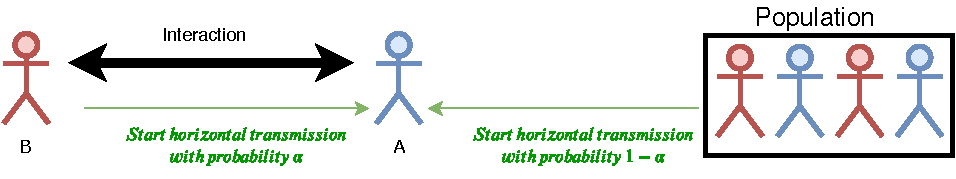
\includegraphics[scale=1]{figure1.pdf}
  \caption{\textbf{Cultural horizontal transmission.} Transmission occurs between interacting partners with probability $\alpha$ (left) or between two random peers with probability $1-\alpha$.}
  \label{fig:horizontal}
\end{figure}
%%%


%%%%%%%%%%%%%%%%%%%%%%%%%%%
%%% Results
\section*{Results}


%%%%%%%%%%%%%%%%%%%%%%%%%%%%%%%%%%%%%%%%%%%%%%%%
\subsection*{Oblique and Horizontal Transmission}

With only oblique and horizontal transmission, i.e. $v = 0$, Eq.\ \ref{eq:horizontal} becomes $\hat{p}=p$ and Eq.\ \ref{eq:nextgen_adults_slimpify} becomes % TODO check this, I changed the ref from nextgen_parents_simplified to nextgen_adults_slimpify
\begin{equation}  \label{eq:nextgen_parents_oblique_only}
p' = p^2 (T_B-T_A) + p (1+T_A-T_B) ,
\end{equation}

which gives the following result.\\

\begin{result}[Oblique and horizontal transmission of cooperation] \label{result:obli_hori}
Without vertical transmission ($v=0$), if there is a horizontal transmission bias in favor of cooperation, namely
\begin{equation} \label{eq:oblique_only_result}
T_A > T_B, 
\end{equation}
then $p'>p$, and the frequency of the cooperator phenotype among adults increases every generation.
\end{result}

Therefore, in the absence of vertical transmission, selection plays no role in the evolution of cooperation. Hence, cooperation will evolve if the cooperator phenotype has a horizontal transmission bias (see~{\autoref{fig:results}c).



%%%%%%%%%%%%%%%%%%%%%%%%%%%%%%%%%%%%%%%%%%
\subsection*{Vertical and Horizontal Transmission}

With only vertical and horizontal transmission, i.e. $v=1$, Eq.\ \ref{eq:horizontal} becomes
$\hat{p} =  \tilde{p}$,
and Eq.\ \ref{eq:nextgen_parents_simplified} for the frequency of the cooperative phenotype among parents in the next generation $\tilde{p}'$ can be written as
\begin{equation} \label{eq:nextgen_parents_vertical_only} 
\begin{aligned}
\bar{w} \tilde{p}' 
& = \tilde{p}^2 (1+b-c) [1 - (1-\tilde{p}) (1-\alpha) T_B] \\
& + \tilde{p}(1-\tilde{p}) (1-c) [\tilde{p} (1-\alpha) T_B + 1 - T_B] \\
& + \tilde{p}(1-\tilde{p}) (1+b) [\tilde{p} (1-\alpha) + \alpha] T_A \\
& + (1-\tilde{p})^2 \tilde{p} (1-\alpha) T_A .
\end{aligned}
\end{equation}

Fixation of either cooperation, $\tilde{p}=1$, or defection, 
$\tilde{p}=0$, are equilibria of Eq.\ \ref{eq:nextgen_parents_vertical_only}, that is, they solve $\tilde{p}'= \tilde{p}$.
We therefore assume for the remainder of the analysis that $0<\tilde{p}<1$.

If $\alpha=1$, then $\tilde{p}'= \tilde{p}$ is reduced to
\begin{equation}
\tilde{p}(1-\tilde{p})\big[(1+b)T_A + (1-c)(1-T_B)-1\big] = 0,
\end{equation}
and there are no additional equilibria.
For cooperation to take over the population (for $\tilde{p}=1$ to be globally stable) we require $\tilde{p}'>\tilde{p}$; that is,
\begin{equation}
  \tilde{p}^2 (1+b-c) + \tilde{p}(1-\tilde{p}) \big[(1-c) (1 - T_B) + (1+b)T_A\big] 
  > \bar{w}\tilde{p} .
\end{equation}
We divide by $\tilde{p}$, set $\bar{w} = 1 + \tilde{p}(b-c)$, and rearrange to get
\begin{equation}
  (1-\tilde{p}) \big[(1-c) (1 - T_B) + (1+b)T_A\big] 
  > 1 -\tilde{p} .
\end{equation}
Dividing by $(1-\tilde{p})$ we find that $\tilde{p}'>\tilde{p}$ if 
\begin{equation} \label{eq:vert_hori_alpha1_condition_proof}
  (1-c) (1 - T_B) + (1+b)T_A
  > 1
\end{equation}
\\

If $\alpha<1$, divide both sides of Eq.\ \ref{eq:nextgen_parents_vertical_only} by $\tilde{p}$ and set $\bar{w} = 1 + \tilde{p}(b-c)$. Then $\tilde{p}'>\tilde{p}$ if
\begin{equation}
\begin{aligned} 
  1 + \tilde{p}(b-c) < 
  & \, \tilde{p}(1+b-c) (1 - (1-\tilde{p}) (1-\alpha) T_B) \\
  & + (1-\tilde{p}) (1-c) (\tilde{p} (1-\alpha) T_B + 1 - T_B) \\
  & + (1-\tilde{p}) (1+b) (\tilde{p} (1-\alpha) + \alpha) T_A \\
  & + (1-\tilde{p})^2 (1-\alpha) T_A .
\end{aligned}
\end{equation}
Rearranging, we get
\begin{equation} 
\begin{aligned} 
  1 - \tilde{p} < 
  & - \tilde{p}(1+b-c)(1-\tilde{p}) (1-\alpha) T_B \\
  & + (1-\tilde{p}) (1-c) (\tilde{p} (1-\alpha) T_B + 1 - T_B) \\
  & + (1-\tilde{p}) (1+b) (\tilde{p} (1-\alpha) + \alpha) T_A \\
  & + (1-\tilde{p})^2 (1-\alpha) T_A .
\end{aligned}
\end{equation}
Diving by $(1-\tilde{p})$ and rearranging so that free terms are on the left and terms with $\tilde{p}$ are on the right, we have
\begin{equation} 
\begin{aligned} 
  &1 - (1-\alpha) T_A - (1+b) \alpha T_A - (1 - T_B)(1-c)  < \\
   &\tilde{p}[ - (1+b-c) (1-\alpha) T_B 
   + (1-c) (1-\alpha) T_B
   + (1+b) (1-\alpha) T_A 
   - (1-\alpha) T_A].
\end{aligned}
\end{equation}
Simplifying, we find that $\tilde{p}'>\tilde{p}$ if and only if
\begin{equation} \label{eq:vert_hori_global_condition}
c(1-T_B) - b \alpha T_A - (T_A-T_B) < \tilde{p} \cdot b (1-\alpha) (T_A-T_B).
\end{equation}

Besides the fixation states $\tilde{p}=0$ and $\tilde{p}=1$, there may be an actual polymorphic equilibrium of $\tilde{p}'=\tilde{p}$ in Eq.\ \ref{eq:nextgen_parents_vertical_only}, namely 
\begin{equation} \label{eq:vert_hori_equilibrium}
  \tilde{p}^* = 
  \frac{c(1-T_B) - b \alpha T_A - (T_A-T_B)}{b (1-\alpha) (T_A-T_B)} ,
\end{equation} 
which is legitimate if $0<\tilde{p}^*<1$.

Since all parameters are positive, we can apply
inequality \ref{eq:vert_hori_global_condition} and see that for $\tilde{p}'>\tilde{p}$ we require that either 
\begin{align} 
\label{eq:vert_hori_global_condition1}
T_A > T_B \quad&\text{and}\quad \tilde{p}>\tilde{p}^*,  \quad \text{or} \\
\label{eq:vert_hori_global_condition2}
T_A <T_B \quad&\text{and}\quad \tilde{p}<\tilde{p}^* .
\end{align}

We summarize these findings in the following result and corollaries.\\

\begin{result}[Vertical and horizontal transmission of cooperation] \label{result:vert_hori}
Without oblique transmission ($v=1$), fixation, extinction, and coexistence of both phenotypes are possible.
\end{result}

Let the initial frequency of the alternative phenotype be $\tilde{p}_0$ and denote the cost boundaries by
\begin{equation} \label{eq:cost_boundaries}
\begin{aligned}
\gamma_1 = \frac{b \alpha T_A + (T_A - T_B)}{1-T_B}, \quad
\gamma_2 = \frac{b \alpha T_B + (1+b) (T_A - T_B)}{1-T_B}.
\end{aligned}
\end{equation}
Then, applying \ref{eq:vert_hori_equilibrium}, \ref{eq:vert_hori_global_condition1}, and \ref{eq:vert_hori_global_condition2}, we  summarize the possible outcomes which are illustrated in \autoref{fig:results2}:
%\begin{enumerate} % p* version
%\item Fixation of cooperation,
%	if $T_A>T_B$ and $0<\tilde{p}^*$, or
%	if $T_A>T_B$ and $0<\tilde{p}^*<1$, and $\tilde{p}_0>\tilde{p}^*$, or
%	if $T_A<T_B$ and $1<\tilde{p}^*$.
%\item Global fixation of defection,
%	if $T_A>T_B$ and $\tilde{p}^*>1$, or
%	if $T_A>T_B$ and $0<\tilde{p}^*<1$, and $\tilde{p}_0<\tilde{p}^*$, or
%	if $T_A<T_B$ and $\tilde{p}^*<0$
%\item Co-existence of both phenotypes at $\tilde{p}^*$, 
%	if $T_A<T_B$ and $0<\tilde{p}^*<1$.
%\end{enumerate}
\begin{enumerate} % gamma version
\item Fixation of cooperation,
	if $T_A>T_B$ and $c<\gamma_1$; or
	if $T_A>T_B$ and $\gamma_1<c<\gamma_2$ and $\tilde{p}_0>\tilde{p}^*$; or
	if $T_A<T_B$ and $c<\gamma_2$.
\item Fixation of defection,
	if $T_A>T_B$ and $\gamma_2<c$; or
	if $T_A>T_B$ and $\gamma_1<c<\gamma_2$ and $\tilde{p}_0<\tilde{p}^*$; or
	if $T_A<T_B$ and $\gamma_1<c$.
\item Coexistence of both phenotypes at $\tilde{p}^*$, 
	if $T_A<T_B$ and $\gamma_2<c<\gamma_1$.
\end{enumerate}

Note that cooperation and defection can  coexist stably if there is horizontal bias for defection and the cost of cooperation is large but not too large. The recursion dynamic for this case is illustrated in \autoref{fig:coexistence}.

Much of the literature on evolution of cooperation focuses on conditions for an initially rare cooperative phenotype to invade a population of defectors.
The next corollary deals with such a condition, followed by a corollary that deals with symmetric horizontal transmission, i.e. $T_A=T_B$.
\\

%%% Figure: Result 2 Boundaries

\begin{figure}[htb]
  \centering
    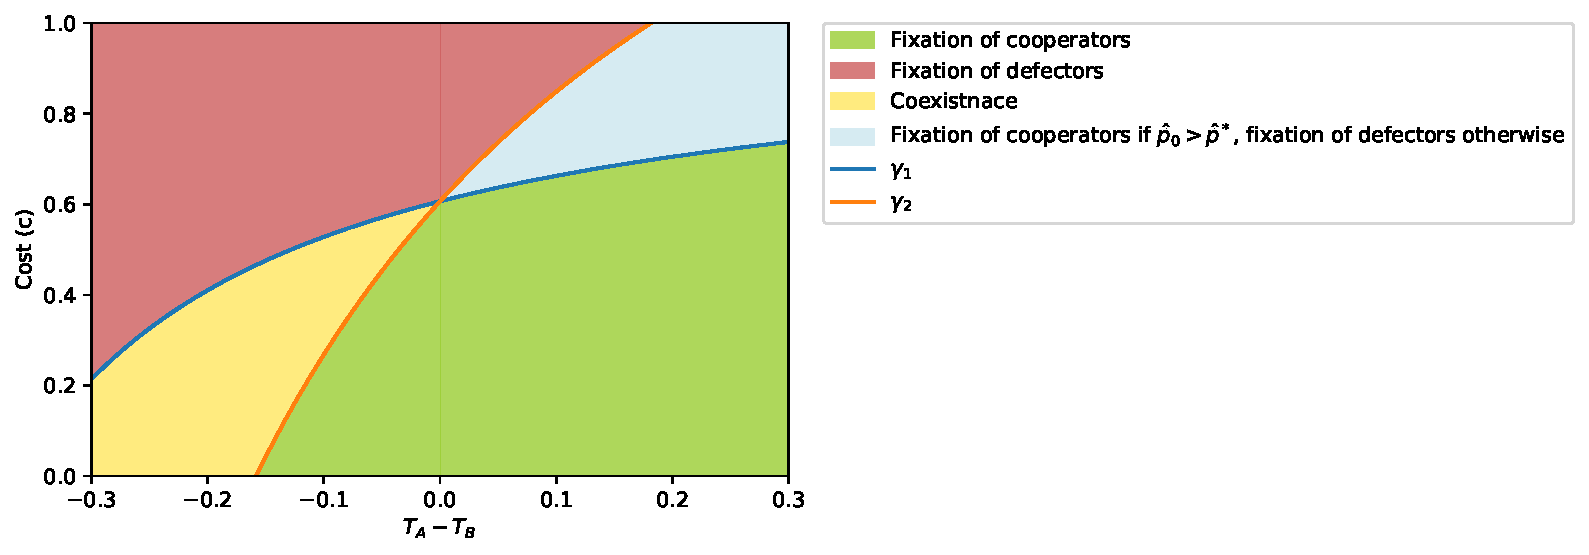
\includegraphics[scale=1]{figure2a.pdf}
    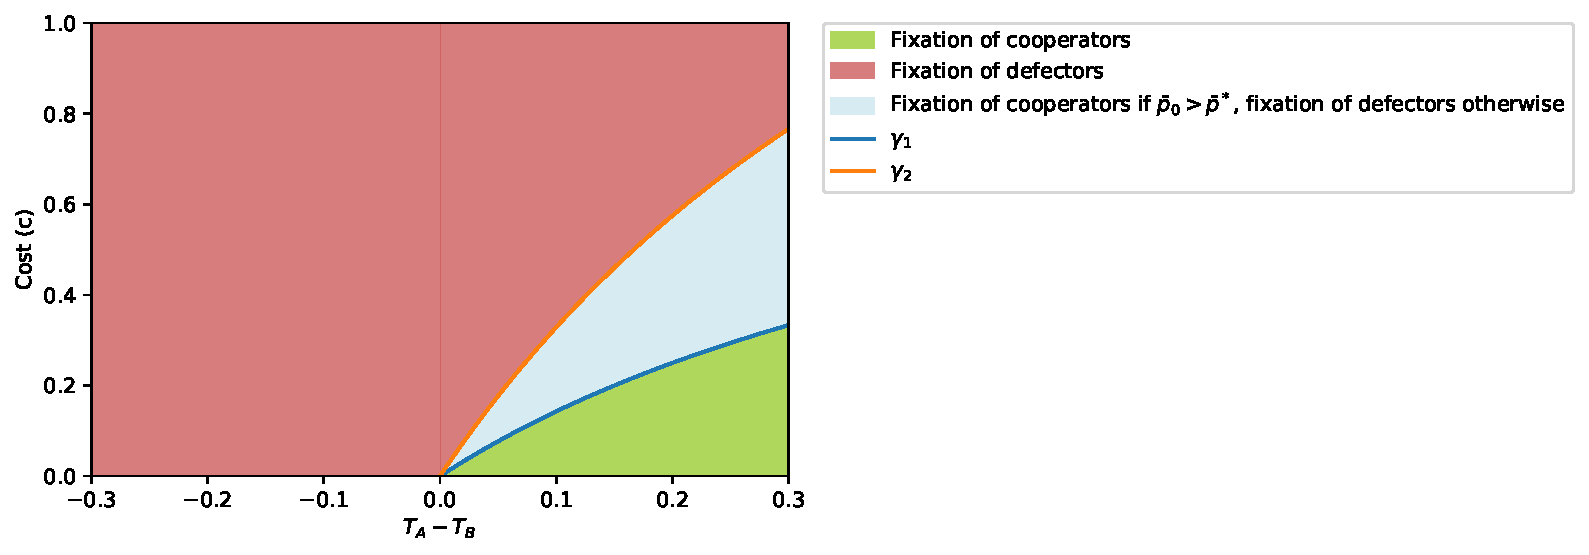
\includegraphics[scale=1]{figure2b.pdf}
  \caption{\textbf{Vertical and horizontal transmission.} The figure illustrates combinations of horizontal bias, $T_A-T_B$, and cost of cooperation, $c$, that lead to either global fixation of cooperation (green), global fixation of defection (red), fixation of either cooperation or defection depending on the initial frequencies (blue), or coexistence of cooperation and defection (yellow). The blue and orange curves show the cost boundaries $\gamma_1$ and $\gamma_2$ (\autoref{eq:cost_boundaries}).
  Here, benefit of cooperation is $b=1.3$, horizontal transmission of cooperation $T_A=0.4$, $c$ and $T_B$ vary on the y- and x-axes. \textbf{Up}: With $\alpha = 0.7 > 0$, coexistence is possible (yellow). \textbf{Down}: With $\alpha=0$, coexistence is not possible.}
    \label{fig:results2}
\end{figure}
%%%

%%% Figure: coexistence map
\begin{figure}[htb]
\centering
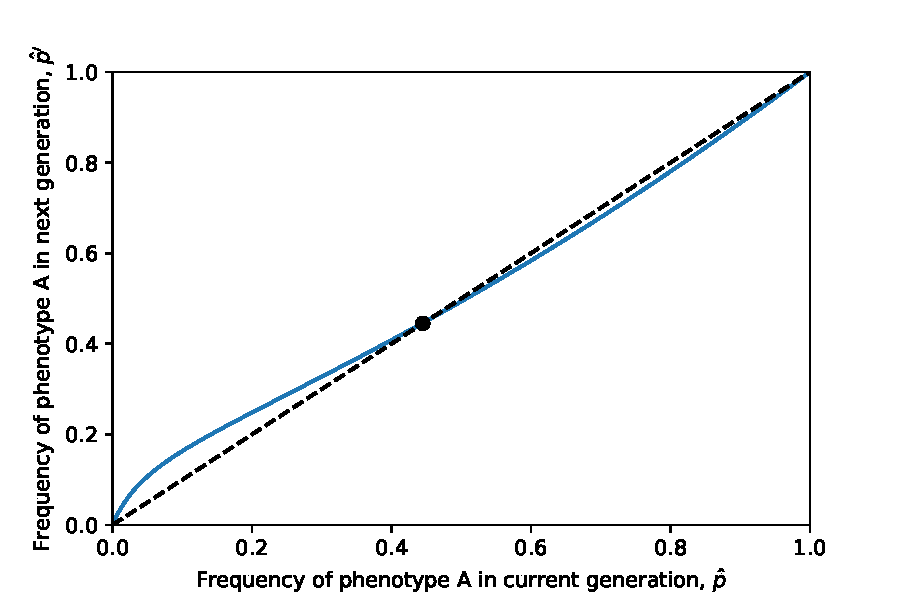
\includegraphics[scale=1]{coexistence.pdf}
\caption{\textbf{Stable coexistence between cooperation and defection.} The frequency of the cooperative phenotype $A$ among juveniles in the next generation $\hat{p}'$ is plotted in blue as a function of the frequency in the current generation $\hat{p}$ for $T_A<T_B$ and $\gamma_2<c<\gamma_1$. The line of $\hat{p}'=\hat{p}$ is in dashed black. The curve and dashed line intersect at the equilibrium $\hat{p}^*$. 
The blue curve is above the black dashed line$\hat{p}<\hat{p}^*$, so that the frequency increases towards $\hat{p}^*$. The blue curve is below the black dashed line when $\hat{p}>\hat{p}^*$, so that the frequency decreases towards $\hat{p}^*$.
}
\label{fig:coexistence}
\end{figure}


\begin{corollary}[Condition for cooperation to increase when initially rare]
If the initial frequency of the cooperative phenotype is very close to zero, $\tilde{p}_0 \approx 0$, then this frequency will increase if 
\begin{equation} \label{eq:unequal_transmission_from_rarity}
\begin{aligned}
T_A>T_B \;\; \text{and} \;\; c < \gamma_1, \quad \text{or} \quad
T_A<T_B \;\; \text{and} \;\; \gamma_2<c < \gamma_1. 
\end{aligned}
\end{equation} 
\end{corollary}

In general, these conditions cannot be formulated in the form of Hamilton's rule ($c<b\cdot r$) due to the horizontal transmission bias $T_A-T_B$.
Without horizontal transmission bias, i.e., with $T_A=T_B$, these conditions reduce to the following  form of Hamilton's rule.\\

\begin{corollary}[Symmetric horizontal transmission]
If $T=T_A=T_B$, then cooperation will take over the population if
\begin{equation}
\label{eq:equal_transmission}
c < b \cdot \frac{\alpha T}{1-T}.
\end{equation}
\end{corollary}
Inequality \ref{eq:equal_transmission} is obtained by setting $T_A=T_B$ in inequality \ref{eq:vert_hori_global_condition} and can be interpreted as a version of Hamilton's rule (inequality \ref{eq:hamilton_rule}), where $\alpha T/(1-T)$ can be regarded as the `effective relatedness'.
\autoref{fig:results}a demonstrates this condition. 
\\

\begin{corollary}[No assortment of transmission and cooperation]
If $\alpha=0$ and there is horizontal bias for cooperation ($T_A>T_B$) and
\textbf{(1)} the cost is low compared to the bias ($c<(T_A-T_B)/(1-T_B)$), then cooperation will fix from any positive frequency; or
\textbf{(2)} the cost is low compared to the benefit ($c<(1+b)(T_A-T_B)(1-T_B)$), then cooperation will fix if the initial frequency is high enough ($\tilde{p}_0 > \tilde{p}^*$).
\end{corollary}

\autoref{fig:results2}b illustrates these conditions, where
 the third equilibrium given by Eq.\ \ref{eq:vert_hori_equilibrium} becomes
\begin{equation} \label{eq:vert_hori_alpha0_equilibrium}
\tilde{p}^*(\alpha=0) = \frac{c(1-T_B) - (T_A-T_B)}{b (T_A-T_B) },
\end{equation} 
and the cost boundaries are
\begin{equation}\begin{aligned}
\gamma_1(\alpha=0) = \frac{T_A - T_B}{1-T_B}, \quad
\gamma_2(\alpha=0) = (1+b)\frac{T_A - T_B}{1-T_B}.
\end{aligned}\end{equation}
If $T_A>T_B$ then $0<\gamma_1(\alpha=0)<\gamma_2(\alpha=0)$.
So either $c<\gamma_1(\alpha=0)$ or $\gamma_1(\alpha=0)<c<\gamma_2(\alpha=0)$ will allow fixation of cooperation, the latter only if the initial frequency is high enough.
If $T_A<T_B$ then $\gamma_2(\alpha=0)<\gamma_1(\alpha=0)<0<c$,
and defection will fix.
%TODO add "effective cost" argument: c<TA-TB/(1-TB) <=> 1-(1-c)(1-TB)<TA.
\\

\begin{corollary}[Complete assortment of transmission and cooperation]
When $\alpha=1$, there are only two equilibria, $\tilde{p}=0$ and $\tilde{p}=1$.
The condition for evolution of cooperation (i.e. global stability of $\tilde{p}=1$) is found from inequality \ref{eq:vert_hori_alpha1_condition_proof}, namely
\begin{equation}\label{eq:vert_hori_alpha1}
c < \frac{b \cdot T_A + (T_A - T_B)}{1-T_B}.
\end{equation}
\end{corollary}
With complete assortment, in inequality \ref{eq:vert_hori_alpha1_condition_proof}
 horizontal transmission  occurs together with the cooperative interaction. The same occurs in \citet{lewin2017microbes}, and therefore this corollary is equivalent to their result (see their eq.~1).

In terms of the cost boundaries, inequality \ref{eq:vert_hori_alpha1} is equivalent to $c<\gamma_1$, and if $T_A>T_B$ then that suffices for fixation of cooperation. If $T_B>T_A$ then $\gamma_2(\alpha=1)<0$ and again, (\ref{eq:vert_hori_alpha1}) is sufficient for increase in the frequency of $A$.
Inequality \ref{eq:vert_hori_alpha1} can be written as
\begin{equation} \label{eq:vert_hori_alpha1_effective}
1 - (1-c)(1-T_B) < (1+b) T_A ,
\end{equation}
which provides an interesting interpretation for the success of cooperation. 
In the interaction between a cooperator and a defector.
$(1-c)(1-T_B)$ is the probability that the cooperator remains cooperative and also reproduces. 
Therefore, $1 - (1-c)(1-T_B)$ is the probability that either the cooperator becomes a defector, or that it fails to reproduce.
This is the effective cost for cooperation from this interaction, while
$(1+b) T_A$ is the probability that the defector becomes cooperative and reproduces, which
 is the effective benefit for cooperation from this interaction.
Thus inequality (\ref{eq:vert_hori_alpha1}) entails that cooperation can evolve if the effective cost for cooperation is less than the effective benefit.


\begin{figure}[htb]
  \centering
    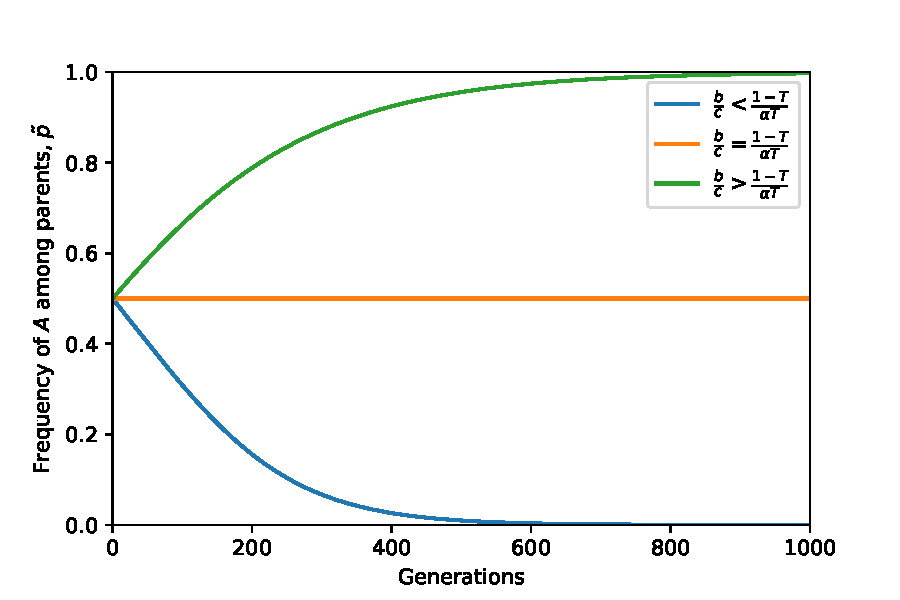
\includegraphics[scale=0.75]{figure3a.pdf}
%    \caption{$v=1$, $T_A=T_B=T$, $\alpha \neq 0$}
  %  \label{fig:results_a}
    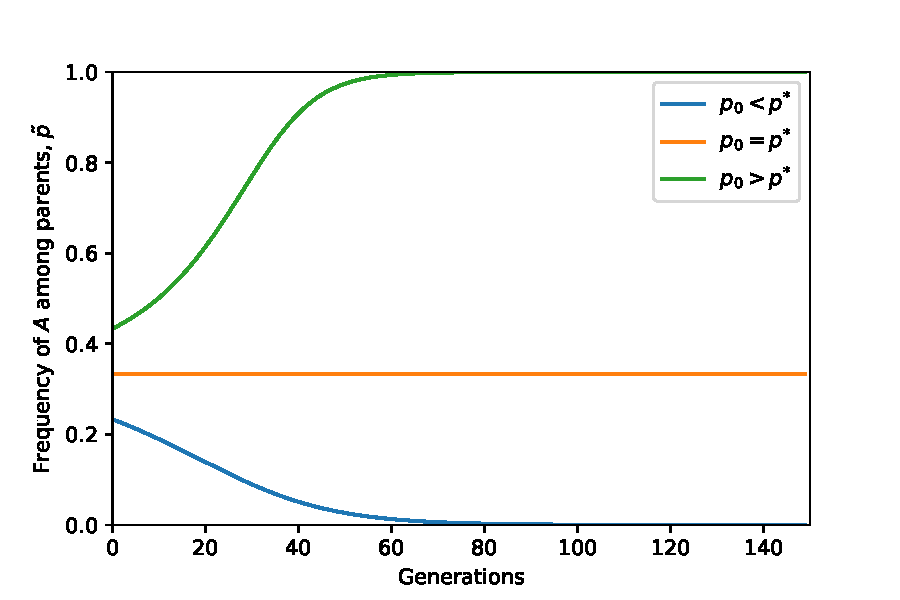
\includegraphics[scale=0.75]{figure3b.pdf}
%    \caption{$v=1$, $\alpha = 0$}
 %   \label{fig:results_b}
    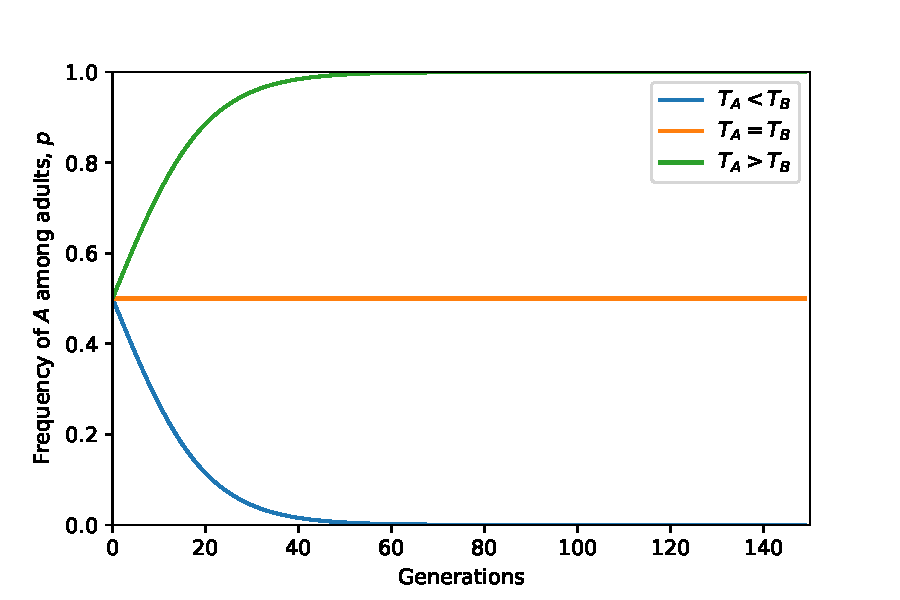
\includegraphics[scale=0.75]{figure3c.pdf}
%    \caption{$v=0$}
%  \label{fig:results}
  \caption{
  \textbf{Numerical results for cultural evolution of cooperation.}
  Shown are dynamics of \textbf{(a-b)} $\tilde{p}$, the frequency of parents with cooperative phenotype $A$; \textbf{(c)} $p$, the frequency of adults with cooperative phenotype $A$.
  The figure demonstrates fixation of cooperation (green), extinction of cooperation (blue), and stable coexistence of cooperators and defectors (orange).
  Parameters: (a) $v=1$, $T_A=T_B=T$, $\alpha \neq 0$; (b) $v=1$, $\alpha = 0$; (c) $v=0$.
  % TODO add all parameters.
  % TODO remove legends, increase fonts, explain in caption instead of legend.
  }
  \label{fig:results}
\end{figure}



%%%%%%%%%%%%%%%%%%%%%%%%%%%%%%%%%%%%%%%%%%%%%%%%
\subsection*{With Vertical and Oblique Transmission}

In this case $0<v<1$, and the recursion system is more complex,
and we focus on local rather than on global stability.
To proceed, we note that 
Eq.\ \ref{eq:horizontal} can give $\hat{p}'$ as a function of both $p'$ and $\tilde{p}'$.
%Equation 4 does not give $\hat{p}$---MF
Eq.\ \ref{eq:nextgen_adults_slimpify} gives $p'$ as a function of $\tilde{p}$, since $\hat{p}$ is given in Eq.\ \ref{eq:horizontal} as a function of $\tilde{p}$ and 
Eq.\ \ref{eq:nextgen_parents_simplified} gives $\tilde{p}'$ as a function of $\hat{p}$. 
Combining these equations, we find an equation for $\hat{p}'$ as a function of $\hat{p}$ (shown in Appendix~\autoref{sec:appendixB}).
We then determine the equilibria, namely, solutions of $\hat{p}' = \hat{p}$, and analyse their local stability.
%: an equilibrium $\hat{p}^*$ is locally stable when the derivative of $f(\hat{p})=\bar{w}(\hat{p}'-\hat{p})$ at the equilibrium is negative, $f'(\hat{p}^*)<0$. 

%We start with the simple case of symmetrical horizontal transmission, $T=T_A=T_B$ and apply \autoref{eq:horizontal}, \autoref{eq:nextgen_adults_slimpify}, and \autoref{eq:nextgen_parents_simplified} to obtain 
%\begin{equation} \label{eq:equal_horizontal_transmission}
%\begin{aligned}
%  f(\hat{p}) &= 
%  \bar{w}(\hat{p}' - \hat{p}) = \\
%  &\hat{p}(1-\hat{p})\big[\alpha bvT - cv(1-T)\big].\end{aligned}
%\end{equation}
%A detailed explain of how we get eq.~\ref{eq:equal_horizontal_transmission} can be found in appendix B.
%The equilibria are solutions of $f(\hat{p})=0$, or $\hat{p}' = \hat{p}$.
%It is easy to verify that fixation of either phenotype, $\hat{p} =  0$ and $\hat{p} = 1$, is an equilibrium.
%Since the derivative of $f'(\hat{p}$ is 
%\begin{equation}
%f'(\hat{p})=(1-2\hat{p})\big[\alpha bvT - cv(1-T)\big],
%\end{equation}
%then the condition for local stability of $\hat{p}=1$ is
%\begin{equation} \label{eq:derivative_of_phattag-phat}
%	f'(1) =	-\alpha bvT + cv(1-T) < 0,
%\end{equation}
%which gives the following result.
%
%\textbf{Result 3: Oblique and vertical transmission with symmetric horizontal transmission.}
%If horizontal transmission is symmetric, $T = T_A = T_B$, and if
%\begin{equation} \label{eq:oblique_and_vertic_result2}
%  %\frac{b}{c}>\frac{1-T}{\alpha T}
%	c < b \cdot \frac{\alpha T}{1-T},
%\end{equation}
%then fixation of the cooperator phenotype $A$ is locally stable.
%The same condition was given in Corollary 1.1, \autoref{eq:equal_transmission}.

%We now turn to the general case where $T_A \neq T_B$. 
We apply Eqs.\ \ref{eq:horizontal}, \ref{eq:nextgen_adults_slimpify}, and \ref{eq:nextgen_parents_simplified} to obtain the function $f(\hat{p})$ (see Appendix~\autoref{sec:appendixB}):

\begin{equation} \label{eq:general_case_polynomial}
  f(\hat{p}) = \bar{w}(\hat{p}'-\hat{p}) =
  \beta_1 \hat{p}^3 + \beta_2 \hat{p}^2 + \beta_3 \hat{p},
\end{equation}
where 
\begin{equation} \label{eq:polynomial_coefficients}
\begin{aligned}
\beta_1 &= \big[c(1-v) - b (1-\alpha v)\big] (T_A-T_B) , \\
\beta_2 &= -\beta_1 -\beta_3 ,  \\
\beta_3 &= \alpha bvT_A - cv(1-T_B) + (T_A-T_B) .
\end{aligned}
\end{equation}

If $T=T_A=T_B$ then $\beta_1=0$ and $\beta_3=-\beta_2=\alpha b vT -cv(1-T)$, 
and $f(\hat{p})$ becomes a quadratic polynomial:
\begin{equation} \label{eq:equal_horizontal_transmission}
  f(\hat{p}) = \hat{p}(1-\hat{p})\big[\alpha bvT - cv(1-T)\big].
\end{equation}
Clearly the only two equilibria are the fixations  $\hat{p} =  0$ and $\hat{p} = 1$.
These equilibria are locally stable if $f'(\hat{p})<0$ near the equilibrium (Appendix~\autoref{sec:appendixC}), and
\begin{equation}
f'(\hat{p})=(1-2\hat{p})\big[\alpha bvT - cv(1-T)\big],
\end{equation}
with
\begin{equation} \label{eq:derivative_of_phattag-phat}
\begin{aligned}
	f'(0) &=	\alpha bvT - cv(1-T), \\
	f'(1) &=	-\alpha bvT + cv(1-T).
\end{aligned}
\end{equation}
Therefore with symmetric horizontal transmission, fixation of the cooperative phenotype ($\hat{p}=1$) occurs under the same condition as Corollary 1.1, namely Eq.\ \ref{eq:equal_transmission}.


In the general case where $T_A \neq T_B$, the coefficient $\beta_1$ is not necessarily zero, and $f(\hat{p})$ is a cubic polynomial.
Therefore, three equilibria may exist, two of which are
$\hat{p} = 0 $ and $\hat{p} = 1$, and the third is
\begin{equation} \label{eq:oblique_and_vertic_result}
  \hat{p}^* =  
  \frac{\beta_3}{\beta_1}.
\end{equation}

Note that the sign of the  cubic (Eq.\ \ref{eq:general_case_polynomial}) at positive (negative) infinity is equal (opposite) to the sign of $\beta_1$. 
If $T_A>T_B$, then 
\begin{equation} \label{eq:beta1}
   \beta_1 < [c(1-\alpha v) - b(1-\alpha v)] (T_A-T_B) 
   = (1-\alpha v)(c-b)(T_A-T_B) < 0 ,
 \end{equation}
since $c<b$ and $1>\alpha v$. Hence the signs of the cubic at positive and negative infinity are negative and positive, respectively.
First, if $\beta_3<\beta_1$ then 
$1<\hat{p}^*$ and therefore $f'(0)<0$ and $f'(1)>0$; that is, fixation of the defector phenotype $B$ is the only locally stable legitimate (i.e. between 0 and 1) equilibrium.
Second, if $\beta_1<\beta_3<0$ then 
$0<\hat{p}^*<1$ and therefore $f'(0)<0$ and $f'(1)<0$, that is, both fixations are locally stable and $\hat{p}^*$ separates the domains of attraction.
Third, if $0<\beta_3$ then 
$\hat{p}^*<0$ and therefore $f'(0)>0$ and $f'(1)<0$; that is, fixation of the cooperator phenotype $A$ is the only locally stable legitimate equilibrium.

Similarly, if $T_B>T_A$, then
\begin{equation} \label{eq:beta1_rev}
   \beta_1 > [c(1-\alpha v) - b(1-\alpha v)] (T_A-T_B) 
   = (1-\alpha v)(c-b)(T_A-T_B) > 0,
 \end{equation}
since $c<b$ and $1>\alpha v$, and the signs of the cubic at positive and negative infinity are positive and negative, respectively. 
First, if $\beta_3<0$ then $\hat{p}^*<0$ and therefore $f'(0)<0$ and $f'(1)>0$; that is, fixation of the defector phenotype $A=B$ is the only locally stable legitimate equilibrium.
Second, if $0<\beta_3<\beta_1$ then $0<\hat{p}^*<1$ and therefore $f'(0)>0$ and $f'(1)>0$; that is, both fixations are locally unstable and $\hat{p}^*$ is a stable polymorphic equilibrium.
Third, if $\beta_1<\beta_3$ then $\hat{p}^*>1$ and therefore $f'(0)>0$ and $f'(1)<0$, and fixation of the cooperator phenotype $A$ is the only locally stable legitimate equilibrium.

The following result summarizes these findings.

\begin{result}[Vertical, oblique, and horizontal transmission of cooperation] \label{result:vert_obli_hori}
The cultural evolution of a cooperator phenotype will follow one of the following scenarios, depending on the horizontal transmission bias $T_A-T_B$ and the coefficients $\beta_1$ and $\beta_3$:
\begin{enumerate}
<<<<<<< HEAD
\item \emph{Fixation of cooperation}, 
if $T=T_A=T_B$ and $c < b\cdot \frac{\alpha T}{1-T}$; or
if $T_A>T_B$ and $0<\beta_3$; or 
if $T_A<T_B$ and $\beta_1<\beta_3$.
\item \emph{Fixation of the defection}, 
if $T=T_A=T_B$ and $c > b\cdot \frac{\alpha T}{1-T}$; or 
if $T_A>T_B$ and $\beta_3<\beta_1<0$; or 
if $T_A<T_B$ and $\beta_3<0$.
\item \emph{Coexistence of both phenotypes at $\hat{p}^*$},
if $T_A < T_B$ and $0<\beta_3<\beta_1$.
\item \emph{Fixation of either phenotype depending on initial frequency}, if $T_A>T_B$ and $\beta_1<\beta_3 < 0$.
=======
\item \emph{Fixation of cooperation}: 
if \emph{(i)} $T=T_A=T_B$ and $c < b\cdot \frac{\alpha T}{1-T}$; or
 \emph{(ii)} if $T_A>T_B$ and $0<\beta_3$; or 
 \emph{(iii)} if $T_A<T_B$ and $\beta_1<\beta_3$.
\item \emph{Fixation of the defection}: 
if \emph{(iv)}  $T=T_A=T_B$ and $c > b\cdot \frac{\alpha T}{1-T}$; or 
 \emph{(v)} if $T_A>T_B$ and $\beta_1<\beta_3<0$; or 
 \emph{(vi)} if $T_A<T_B$ and $\beta_3<0$.
\item \emph{Coexistence of both phenotypes at $\hat{p}^*$}: 
if \emph{(vi)} $T_A < T_B$ and $0<\beta_3<\beta_1$.
\item \emph{Fixation of either phenotype depending on initial frequency}: if \emph{(vii)}  $T_A>T_B$ and $\beta_3<\beta_1$.
>>>>>>> e545160... marck changes

\end{enumerate}
\end{result}

%%%%%%%%%%%%%%%%%%%%%%%%%%%
% Discussion
\section*{Discussion}
We hypothesized that non-vertical transmission can explain the evolution of cooperation and evaluated this hypothesis using a deterministic discrete-time evolutionary model with fitnesses in the form of payoffs from a prisoner's dilemma game..
Under oblique and horizontal transmission, horizontal transmission bias for the cooperative phenotype was found to be sufficient and necessary for evolution of cooperation (Result~\autoref{result:obli_hori}).
Under horizontal and vertical cultural transmission, cooperation, or defection can fix, or coexist at a stable polymorphism, depending on the relationship between the cost and benefit of cooperation, the horizontal bias, and the correlation between cooperation and transmission (Result~\autoref{result:vert_hori}).
Under a combination of vertical, oblique, and horizontal transmission the dynamics are much more complicated. However, we show that under some conditions cooperation can evolve, and can even be maintained in  stable coexistence with defection (Result~\autoref{result:vert_obli_hori}).

This study was partially inspired by the work of \citet{lewin2017microbes}, 
who hypothesised that microbes that manipulate their hosts to act altruistically can be favored by selection, and may play a role in the widespread occurrence of cooperative behavior. Indeed, it has been shown that microbes can mediate behavioral changes in their hosts~\citep{dobson1988population,poulin2010parasite}. Therefore, natural selection on microbes may favor manipulation of the host so that it cooperates with others. Microbes can be transmitted \emph{horizontally} from one host to another during host interactions, and following horizontal transfer, the recipient host may carry microbes that are closely related to the microbes of the donor host, even when the two hosts are (genetically) unrelated~\citep{lewin2017microbes}. Microbes can also be transferred vertically, from parent to offspring, and % yr: cite 10.1126/science.aat7164
a microbe that induces its host to cooperate with another host, and thereby increases the latter's fitness, will  increase its vertical transmission  from the receiving individual. Kin selection among microbes could therefore favor those that induce cooperative behavior in their hosts, thereby increasing the transmission of their microbial kin.

%There is an ongoing debate about the extent to which kin selection explains the evolution of cooperation and altruism.
%For example, it has been suggested that it can explain the cooperative behavior of worker castes of eusocial insects like the honey bee. % TODO REF
%The most significant argument against kin selection is that in some cases cooperation among unrelated individuals appears to have evolved~\citep{wilson2005kin}.
%Therefore, other theories have been develop to explain the evolution of cooperation and altruism.

%\emph{Reciprocity} entails that repeated interactions or individual recognition are key components of the evolution of cooperation. In \emph{direct reciprocity} there are repeated encounters between the same two individuals, and at every encounter each individual has a choice between cooperation and defection. Hence, it may eventually pay off to cooperate if it may cause your partner to cooperate in the future.
%This game-theoretic framework, known as the \emph{repeated prisoner's dilemma}, 
%%A well known strategy to play this game is called  'tit-for-tat'. This strategy always starts with a cooperation, then it does whatever the other player has done in the previous round: a cooperation for a cooperation, a defection for a defection. There a unlimited number of possible strategies to play this game. However, 
%can only lead to the evolution of cooperation if the cost is less than the benefit $b$ times the probability of another encounter between the same two individuals, $w$, 
%%TODO Referencess
%\begin{equation} \label{eq:reciprocity}
%c < b \cdot w.
%\end{equation}
%
%Direct reciprocity assumes that both players are in a position to cooperate, but it can not explain cooperation in asymmetric interactions such as human philanthropy. \\
%\emph{Indirect reciprocity} has also been suggested to explain the evolution of cooperation.
%\citet{nowak2006five} claims that direct reciprocity is like a barter economy based on the immediate exchange of goods, while indirect reciprocity resembles the invention of currency. 
%%TODO: refs
%The currency that ``fuels the engines'' of indirect reciprocity is \emph{reputation}. 
%However, reciprocity assumes repeated interactions and therefore has difficulty in explaining the evolution of cooperation if  interactions are not repeated. 
%
%\emph{Group selection} theory posits that cooperation is favored because it imparts an advantage to the whole group, if selection acts at the group level in addition to the individual level. A common model for group selection divides the population into groups in which there are cooperators that help  other group members and defectors that do not.  % TODO add reference
%Individuals reproduce proportionally to their fitness, and offspring are added to the same group as their parents.
%If a group reaches a certain size it can split to two groups, so groups that grow faster will split more often.
%Groups with cooperators grow faster than groups without cooperators, and
%cooperation can evolve in this model when the cost $c$ is less than the benefit $b$ times the ratio between the  the number of groups $m$ and the sum of $m$ and the maximum group size $n$,
%\begin{equation} \label{eq:groupselection}
%c < b \cdot \frac{m}{m+n} .
%\end{equation}
%
%Group selection has been criticized by biologists who advocate a gene-centered view of evolution. % TODO ref
%It has also been criticized because for cooperation to take over the population it must have higher fitness than defection, while under group selection theory the fitness of cooperators at the individual level is lower than the fitness of defectors. Thus a trait with a lower fitness taking over the population is a contradiction %TODO ref.
%\citet{eldakar2011eight} reject this argument, claiming that it is a tautology and does not qualify as an argument against group selection. The distinction between individual and group selection requires a comparison of fitness differentials within and between groups in a multi-group population, and when a trait  evolves by group selection, despite having lower fitness within a group, that group might have higher average fitness in competition with other groups, all things considered. % TODO cite Simpsons' paradox?

\citet{Eshel1982}  showed that with assortative meeting, namely, a probability $m$ that individuals interact  within their phenotypic group, cooperation can evolve if $c < b \cdot m$.
Our results highlight another possibility for assortative meeting, namely, individuals interacting at rate $\alpha$ with their cultural partners, resulting in horizontal transmission.
We show that high levels of assortative meeting  significantly increase the potential for evolution of cooperation. With a high enough $\alpha$, cooperation can increase when initially rare (although it will not fix) even when there is horizontal bias against cooperation ($\alpha > \big(c(1-T_B) + (T_B-T_A)\big) / b T_A$, see Result~\autoref{result:vert_hori})

An important implication of our results is that cooperation can evolve even in a fully mixed population (i.e., in an unstructured population), without repeated interactions or individual recognition.
This highlights the potential importance of non-vertical cultural transmission for explaining complex evolutionary phenomena, and  furthers our understating of the cultural evolution of cooperation. 

% Javarone MA, Atzeni AE, Galam S. Emergence of Cooperation in the Prisoner ’ s Dilemma Driven by Conformity. 2:155-163. doi:10.1007/978-3-319-16549-3
% Woodcock S. The significance of non-vertical transmission of phenotype for the evolution of altruism. Biol Philos. 2006;21:213-234. doi:10.1007/s10539-005-8241-1


%%%%%%%%%%%%%%%%%%%%%%%%%%%
%\pagebreak
% Acknowledgements
{\small
\section*{Acknowledgements}
We thank Lilach Hadany and Ayelet Shavit for discussions and comments.
This work was supported in part by
the Israel Science Foundation 552/19 (YR),
and Minerva Stiftung Center for Lab Evolution (YR).
% TODO funding for other authors?
}







%%%%%%%%%%%%%%%%%%%%%%%%%%%
% Appendices
\begin{appendices}
\renewcommand{\theequation}{\thesection\arabic{equation}}
\counterwithin*{equation}{section}

%%%%%%%%%%%%%%%%%%%%%%%%%%%%%%%%%%%%%%%%%%%%%%%%%%%%%
\section{} \label{sec:appendixB}
We want to find the frequency of juveniles with phenotype $A$ in next generation $\hat{p}'$ as a function of frequency
of juveniles with phenotype $A$ in the current generation $\hat{p}$.
Starting from \autoref{eq:horizontal},
\begin{equation}\label{eq:appendix_b_1}
  \hat{p}' = v \tilde{p}' + (1-v) p',
\end{equation}
we substitute $p'$ using \autoref{eq:nextgen_adults_slimpify} and $\tilde{p}'$ using \autoref{eq:nextgen_parents_simplified}, we have
\begin{equation}\label{eq:appendix_b_2}
  \begin{aligned}
  \hat{p}'  = & \frac{v}{\bar{w}}\left\{\hat{p}^2(1+b-c)\left[1-(1-\hat{p})(1-\alpha)T_B)\right]\right\} \\
  & + \frac{v}{\bar{w}}\left\{ \hat{p}(1-\hat{p})(1-c)\left[ \hat{p}(1-\alpha)T_B + 1 - T_B \right] \right\} \\
  & + \frac{v}{\bar{w}}\left\{ \hat{p}(1-\hat{p})(1+b)\left[\hat{p}(1-\alpha) + \alpha \right]T_A \right\} \\
  & + \frac{v}{\bar{w}}(1-\hat{p})^2\hat{p}(1-\alpha)T_A \\
  & + (1-v)\hat{p}^2(T_B-T_A) + (1-v)\hat{p}(1+T_A-T_B),
\end{aligned}
\end{equation}
where $\bar{w} = 1 + \hat{p}(b-c)$. 
We define $f(\hat{p})$ as
\begin{equation} \label{eq:appendix_define_f}
\begin{aligned}
      f(\hat{p}) &= \bar{w}(\hat{p}' - \hat{p})
\end{aligned}
\end{equation}
Using \emph{SymPy} \citep{Meurer2017}, a Python library for symbolic mathematics, we simplify \autoref{eq:appendix_define_f} to 
eqs.~\ref{eq:general_case_polynomial}-\ref{eq:polynomial_coefficients}.

%%%%%%%%%%%%%%%%%%%%%%%%%%%%%%%%%%%%%%%%%%%%%%%%%%%%
\section{} \label{sec:appendixC}

Denote $f(p)=\lambda(p'-p)$, where $\lambda>0$, and assume $f(p^*)=0$; i.e., $p^*$ is an equilibrium.
%HOW DO YOU KNOW $p^*\in(0,1)$?--MF
We want a condition for $|p'-p^*| < |p-p^*|$.

If $p>p^*=0$, we want a condition for $p'<p$, or
$\frac{p'}{p}<1$, or
$\lambda \frac{p'-p}{p} < 0$, or
$\frac{f(p)}{p} < 0$.
Using a linear approximation for $f(p)$ near $0$, we have
\begin{equation}\begin{aligned}
p' &< p \Leftrightarrow \\
\frac{f'(0) \cdot p + O(p^2)}{p} &< 0 \Leftrightarrow \\
f'(0) + O(p) &< 0.
\end{aligned}\end{equation}
Therefore, by definition of big-O notation, if $f'(0)<0$ then there exists $\epsilon>0$ such that for any $0<p<\epsilon$, it is guaranteed that $0<p'<p$, that is, $p'$ is closer than $p$ to zero.

If $p<p^*=1$, we want a condition for $1-p' < 1-p$, or
$\frac{1-p'}{1-p}<1$, or
$\lambda \frac{-(p'-p)}{1-p} < 0$, or
$-\frac{f(p)}{1-p} < 0$.
Using a linear approximation for $f(p)$ near $1$, we have
\begin{equation}\begin{aligned}
1-p' &< 1-p  \Leftrightarrow \\
\frac{f'(1)(p-1) + O\big((p-1)^2\big)}{p-1} &< 0 \Leftrightarrow \\
f'(1) - O(1-p) &< 0.
\end{aligned}\end{equation}
Therefore, if $f'(1)<0$ then there exists $\epsilon>0$ such that for any $1-\epsilon<1-p<1$ it is guaranteed that $1-p'<1-p$, that is, $p'$ is closer than $p$ to one.


\end{appendices}

%%%%%%%%%%%%%%%%%%%%%%%%%%%
% Bibliography
\bibliographystyle{plainnat}
\bibliography{bib}

\newpage

\begin{table}[h]
\centering
\begin{tabular}{lll}
\toprule
           & $\phi_2=A$ & $\phi_2=B$ \\ \cmidrule(r){1-3}
$\phi_1=A$ & $1+b-c$ & $1-c$ \\
$\phi_1=B$ & $1+b$   & $1$
\\ \bottomrule
\end{tabular}
\caption{\textbf{Payoff matrix for prisoner's dilemma.}
The fitness of phenotype $\phi_1$ when interacting with phenotype $\phi_2$. $A$ is a cooperative phenotype, $B$ is a defector phenotype, $b$ is the benefit gained by an individual interacting with a cooperator, and $c$ is the cost of cooperation. $b>c>0$.
}
\label{table:prisoner_payoff}
\end{table}

\newpage

\begin{table}[]
\begin{tabular}{@{}llllll@{}}
\toprule
\multirow{2}{*}{Phenotype $\phi_1$} &
  \multirow{2}{*}{Phenotype $\phi_2$} &
  \multirow{2}{*}{Frequency} &
  \multirow{2}{*}{Fitness of $\phi_1$} &
  \multicolumn{2}{l}{$P(\phi_1=A)$ via horizontal transmission:} \\ \cmidrule(l){5-6} 
    &     &                      &         & from partner, $\alpha$ & from population, $(1-\alpha)$ \\ \cmidrule(r){1-6}
$A$ & $A$ & $\hat{p}^2$          & $1+b-c$ & 1                      & $\hat{p}+(1-\hat{p})(1-T_B)$  \\
$A$ & $B$ & $\hat{p}(1-\hat{p})$ & $1-c$   & $1-T_B$                & $\hat{p}+(1-\hat{p})(1-T_B)$  \\
$B$ & $A$ & $\hat{p}(1-\hat{p})$ & $1+b$   & $T_A$                  & $\hat{p} T_A$                 \\
$B$ & $B$ & $(1-\hat{p})^2$      & $1$     & $0$                    & $\hat{p} T_A$                 \\ \bottomrule
\end{tabular}
\caption{\textbf{Interaction frequency, fitness, and transmission probabilities.}}
\label{table:interactions}
\end{table}
%%%
%%%
\end{document}